\begin{multicols}{2}
        \centering $\text{MCFND}(\hat{d}_1 = 15)$ \vspace{2mm}
    
        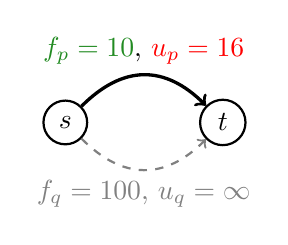
\begin{tikzpicture}[node distance={20mm}, thick, main/.style = {draw, circle}]
            \node[main] (s) {$s$}; 
            \node[main] (t) [right of=s] {$t$};
            \draw[->, very thick] (s) to [out=45, in=135, looseness=1.2] node[midway, above] { {\color{ForestGreen}$f_p = 10$}, {\color{Red} $u_p = 16$}} (t); 
            \draw[->, draw=gray, dashed] (s) to [out=-45, in=-135, looseness=1.2] node[midway, below] { {\color{gray} $f_q = 100$}{\color{gray}, $u_q = \infty$}}(t); 
        \end{tikzpicture} 
        
        \red{$\text{Cost}_1 = 10$}
    
        \columnbreak
        
        \centering 
        $\text{MCFND}(\hat{d}_2 = 17)$\vspace{2mm}
    
        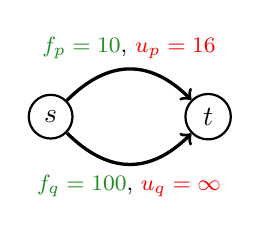
\begin{tikzpicture}[node distance={20mm}, thick, main/.style = {draw, circle}]
            \node[main] (s) {$s$}; 
            \node[main] (t) [right of=s] {$t$};
            \draw[->, very thick] (s) to [out=45, in=135, looseness=1.2] node[midway, above] {\footnotesize {\color{ForestGreen}$f_p = 10$}, {\color{Red} $u_p = 16$}} (t); 
            \draw[->, very thick] (s) to [out=-45, in=-135, looseness=1.2] node[midway, below] {\footnotesize {\color{ForestGreen}$f_q = 100$}, {\color{Red} $u_q = \infty$}} (t); 
        \end{tikzpicture} 
    
        {\color{red} $\text{Cost}_2 = 110$}
    \end{multicols}